\documentclass[crop,tikz]{standalone}% 'crop' is the default for v1.0, before it was 'preview'
\usepackage{tikz}
\usetikzlibrary{shapes}
\usetikzlibrary{arrows}
\usetikzlibrary{positioning}
\usetikzlibrary{calc}
\usetikzlibrary{fit}
\usetikzlibrary{backgrounds}
\usetikzlibrary{shadows}
\usepackage{placeins}
\usepackage{amsmath,amssymb,amsfonts}
\usepackage[mathscr]{euscript}
\begin{document}

	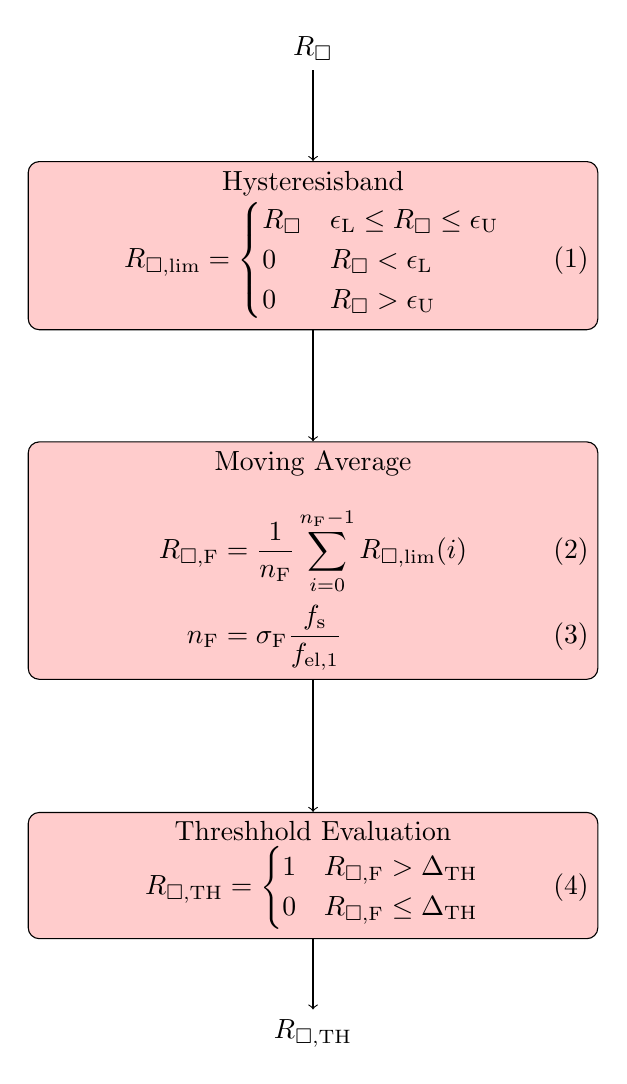
\begin{tikzpicture}
	\def\minipagew{7cm}
	\tikzstyle{box} = [rectangle, rounded corners, minimum height=1cm, text centered, draw=black, align=center,fill=red!20]
	\tikzstyle{retransform} = [minimum width=2cm]
	\tikzstyle{sum} = [circle, minimum height=0.1cm, draw=black]
	\tikzstyle{contr} = [box, minimum width=1cm]
	\tikzstyle{park} = [box, minimum width=2cm]
	\node (entry)[] at (0, 2.5) {$R_\square$};
	\node (hysteresis)[box] at (0, 0) {Hysteresisband\\
		\begin{minipage}{\minipagew}
			\begin{equation}
				R_{\square\textrm{,lim}} =
				\begin{cases}
					R_\square & \epsilon_\textrm{L} \leq R_\square \leq \epsilon_\textrm{U} \\
					0 & R_\square < \epsilon_\textrm{L} \\
					0 & R_\square > \epsilon_\textrm{U}
				\end{cases}\label{eq:R_hysteresis}
			\end{equation}
		\end{minipage}
	};
	\node (filter)[box] at (0, -4) {Moving Average\\
		\begin{minipage}{\minipagew}
			\begin{align}
				R_{\square\textrm{,F}} &= \frac{1}{n_\textrm{F}}\sum\limits_{i=0}^{n_\textrm{F}-1} R_{\square\textrm{,lim}}(i)  \label{eq:R_filter}\\
				n_\textrm{F} &= \sigma_\textrm{F} \frac{f_\textrm{s}}{f_\textrm{el,1}} \label{eq:filterlength}
			\end{align}
		\end{minipage}
	};
	\node (threshold)[box] at (0, -8) {Threshhold Evaluation\\
		\begin{minipage}{\minipagew}
			\begin{equation}
				R_{\square\textrm{,TH}} =
				\begin{cases}
					1 & R_{\square\textrm{,F}} > \Delta_\textrm{TH} \\
					0 & R_{\square\textrm{,F}} \leq \Delta_\textrm{TH}
				\end{cases}\label{eq:R_threshold}
			\end{equation}
		\end{minipage}
	};
	\node (exit)[] at (0, -10) {$R_{\square\textrm{,TH}}$};
	\draw[->] (entry.south) -- (hysteresis.north);
	\draw[->] (hysteresis.south) -- (filter.north);
	\draw[->] (filter.south) -- (threshold.north);	
	\draw[->] (threshold.south) -- (exit.north);
\end{tikzpicture}
\end{document}